% Users can also go through the FAQs available on the journal's submission webpage.
%
% Steps to compile: latex, bibtex, latex latex
%
% For tracking purposes => this is v1.3 - May 2012


\documentclass{acmlarge-edm}

% Metadata Information
\acmVolume{1}
\acmNumber{2}
\acmArticle{3}
\acmYear{2012}
\acmMonth{5}  % can also put in literal name

\usepackage{graphics}

% Metadata Information would go here

% Document starts
\begin{document}


% Title portion
\title{Models of student learning and multimodel inference}
\author{Brett van de Sande
\affil{Arizona State University\\bvds@asu.edu}}

%
%  Cool LaTeX resource:
%   http://en.wikibooks.org/wiki/LaTeX

\begin{abstract}
We compare several models of student learning with the goal of
determining when a specific student has learned a particular skill.
We use Likelihood Theory to determine which of several models best
describes the acquisition of skills associated with introductory
physics.  Then we use a multimodel approach to determine the relative
probability that a student has learned a given skill at a particular
problem-solving step.
\end{abstract}

%\category{C.2.2}{Computer-Communication Networks}{Network Protocols}

%\terms{Design, Algorithms, Performance}

\keywords{data mininig, models of student learning}

%\acmformat{Zhou, G., Wu, Y., Yan, T., He, T., Huang, C., Stankovic,
%J. A., and Abdelzaher, T. F.  2010. A multifrequency MAC specially
%designed for  wireless sensor network applications.}

\begin{bottomstuff}
Funding for this research was provided by the Pittsburgh Science of
Learning Center which is funded by the National Science Foundation
award No. SBE-0836012.
\end{bottomstuff}


\maketitle


\section{Introduction}

%Talk about ultimate goal of using this to determine effectiveness
%of help given or of a particular student behavior.

The traditional experimental paradigm for studying student learning
is to use a pre-test and post-test combined with two or more experimental
conditions.  Pre-test and post-test scores can indicate {\em whether}
learning has occurred, but not {\em when} it may have occurred.  In a
multi-condition experiment, one can see if a particular change
to the instructional materials or help-giving strategy results in 
greater learning.  However, this way of doing things does not directly measure whether
any changes in student {\em behavior} results in greater learning.
Also, in a more realistic setting, such as in an {\em in vivo}
study~\cite{in-vivo}, there is relatively little control over what
happens during the experimental intervention and there is necessarily
an extended time between the the pre-test and post-test.  Thus, in
cases where the intervetion is applied briefly, any
experimental ``signal'' can easily be swamped by these uncontrolled effects.

%Talk about micky chi paper with relative infrequency of well-defined 
%Aha moments.

However, in a more realistic setting, such as a
classroom, the experimenter is faced with a number of obstacles:
first

There is ample evidence that a well-designed Intelligent Tutor System
(ITS) can be almost as effective as an expert human
tutor~\cite{vanlehn_relative_2011}.  A key ingredient for improving an
ITS is determining whether a particular student action or the tutoring
given by the ITS at a given instance was effective.  There are several
senses in which an activity might be ``effective.''  For instance:
%
\begin{itemize}
\item Did it improve the student's attitude toward
the subject?  
\item Did it minimize time-on-task (assuming 
a skill was eventually learned)?  
\item Did it improve the student's 
problem-solving skills?  
\item Did it prepare the student to learn
material later in the course?
\end{itemize}

In the present investigation, we will take a narrower definition
of effectiveness of a particular student or tutor action:  
Did the action immediately precede the
student learning a new skill?  Answering this question requires
the use of some sort of embedded assessment of student learning.
Presumably, a student will encounter a given skill multiple times
during a problem solving session, so any pre-test/post-test will
not tell us directly at what step the student learned the skill
(although the effectiveness of a particular action can
be experimentally inferred by conducting a two-condition study).
In addition, it means that the determination must be made
after the fact, typically through some log file analysis. 

In this work, we investigate a method for determining when a student
may have learned a skill based on their ability to apply that skill
without errors or asking for hints.  In principle, there are other
observables that may give us clues on mastery: for instance, how much
time a student takes to complete a step.  However, other such
observables need some additional interpretation ({\em exempli gratia,}
How long is too long?).  Baker, Goldstein, and
Heffernan~\citeyear{baker_detecting_2010} attempt a model of learning
based on a Hidden Markov model approach.  In their model, they
consider additional variables.  Inclusion of such additional
observables is a natural extension of the approach we will present
here.

First we will compare three different models of learning and examine
whether there is emphirical support for using one model over the
others.  In fact, using Akaike Information Criteria (AIC), we obtain
results that seem to favor two models over the third, but conclude
that there are some unresolved issues.

Second, we select a model and use a multimodel approach to predict
where learning has occurred, with what probability, and how much
learning has occurred.  We apply our approach to student data and
discuss the reliability of our predictions.


\subsection{Correct/Incorrect steps}

Although there are other observables that may be used
to determine whether a skill has been mastered, Table~1 of
\cite{baker_detecting_2010} list 14 different observables.  
However, we will focus on correctness of a step.  Thus, we need to
define precisely what we mean by a step being correct.

For each student and Knowledge Component (KC)~\cite{vanlehn_behavior_2006}, 
the student has attempted some number of 
{\em steps} that involve that KC.   We will label
steps with $j\in\left\{1,\ldots,N\right\}$.  
Usually a given step is associated
with a single user interface object (an equation, vector, etc.)  but
not always, since a student may attempt a particular problem solving
step, delete the object, and later attempt that solution step again.
Sometimes, we talk of a step being an {\em opportunity} to learn
a given skill if the student needs to apply that skill
to complete that step.

%
%  Not needed in this paper.
%
%Each step $j$ corresponds some some number of student-tutor 
%{\em transactions}: attempts at constructing the associated object, 
%or associated interactions with the Andes help system.  

%Next, we need a model of student learning for a particular KC.
%Since the policies chosen by the random-help version of Andes
%are different for each student,
%we need to determine the point of learning for each student.
For each KC and student, mark each step as ``correct'' if
the student completes the step correctly without any associated errors or 
requests for help; otherwise, the step is marked as ``incorrect.''
\label{steps} 
%
% From Kurt:
Thus, if each incorrect/correct step is marked with a 0/1, then
a single student's performance on a single KC is a bit string,
{\em exempli gratia} 00101011.

\section{Three models of learning}

\begin{figure}
  \centering 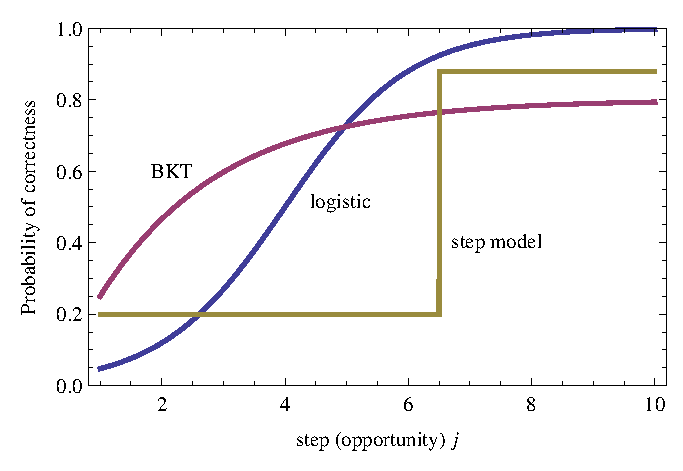
\includegraphics{three-models.eps}
  \caption{Functional form of the three models of student learning.}
    \label{three-models}
\end{figure}


In order to determine when a student has learned a particular still,
we need to introduce a model of learning for that student and skill.
Ideally, the model should have the the following properties:
\label{model-criteria}
%
\begin{enumerate} 

\item Be compatible with actual student behavior.
      That is, its
      functional form should fit well with student data.
      We will explore this question in Section~\ref{model-selection}.  

\item \label{crit:step}
      Give the probability that learning has occurred at a given step.
      We will address this issue in Section~\ref{multi-model}.

\item  \label{crit:perform}
     Assuming learning has occurred at a given step, the model
     should give an prediction for the 
     associated increase in performance and 
     the rate of errors after learning.

\end{enumerate}
%
We will consider three candidate models:  the ``step model,'' 
the logistic function, and the Bayesian Knowledge Tracing model;
see Fig.~\ref{three-models}.


The first model is the Bayesian Knowledge Tracing (BKT) 
model~\cite{corbett_knowledge_1994}.  The hidden Markov model
form of BKT is often fit to student performance 
data~\cite{beck_identifiability:_2007}.  One can show that
this model, in functional form, is an exponential function
with three model parameters~\cite{van_de_sande_properties_2012}:
%
%  A and \beta are kind of messy, so we don't include them here.
\begin{equation}
         P_\mathrm{BKT}(j) = 1-P(S) -A e^{-\beta j} \; .
\end{equation}
%
One central assumption of BKT is that, given that learning
has not already occurred, mastery is {\em equally probable} on each step.
This assumption of equal probability does not match well with 
our goal of determining empirically the steps where learning has 
actually occurred for an individual student, criterion~\ref{crit:step}.
On the other hand, this model does provide initial and final
error rates, so criterion~\ref{crit:perform} is satisfied. 

Another model that is frequently used in the context of learning is
the logistic
model~\cite{cen_learning_2006,chi_instructional_2011},
%
\begin{equation}
    P_\mathrm{logistic}(j)= \frac{1}{1+\exp\left(-b (j-L)\right)} \; .
\end{equation}
%
It is natural to associate $L$ with the moment of learning.  However,
the finite slope $P_\mathrm{logistic}(j)$ means that learning may
occur in a range of roughly $1/b$ steps before and after $L$.  For
$P_\mathrm{logistic}(j)$, the gain in performance is always 1 and the
final error rate is always 0.  Thus, although this model makes a
prediction for when the skill is learned, criterion~\ref{crit:step},
it does not predict a gain in performance,
criterion~\ref{crit:perform}.

The third model is the ``step model'' which assumes that learning 
occurs all at once~\cite{baker_detecting_2011}.  It is defined as:
%
\begin{equation}
    P_\mathrm{step}(j)= \left\{\begin{array}{cc}
                 g, & j<l \\
                 1-s, & j\ge L 
                 \end{array} \right. 
\end{equation}
%
where $L$ is the step where the student first shows mastery of the KC,
$g$ is the ``guess rate,'' the probability that the student gets a
step correct by accident, and $s$ is the ``slip rate,'' the chance
that the student makes an error after learning the skill.  These are
analogous to the guess and slip parameters of
BKT~\cite{corbett_knowledge_1994}.  The associated gain in performance
is $1-g-s$ and the error rate after learning is simply $s$ in this
model.  Thus, this model satisfies criteria \ref{crit:step} and
\ref{crit:perform}.

\section{Model selection using AIC}
\label{model-selection}

Although this will not determine our choice of model in subsequent
work, it would be reassuring to know whether the step model
$P_\mathrm{step}(j)$ describes the student data as well (or better
than) the other two models, $P_\mathrm{logistic}(j)$ and
$P_\mathrm{BKT}(j)$.  We believe that the Akaike Information Criterion
(AIC) is the most appropriate
metric~\cite{akaike_new_1974,burnham_model_2002} to use for this
purpose.  AIC is defined as
%
\begin{equation}
   \mathrm{AIC}= -2 \log\left(\mathcal{L}\right) + 2K
\end{equation}
% 
where $\mathcal{L}$ is the maximized value of the likelihood function
and $K$ is the number of parameters in the model.
 AIC is an estimate of the expected relative distance 
between a given model and the true model (assumed to be complicated) 
that actually generated the observed data.  It is valid in limit of 
many data points, $N\to\infty$, with leading corrections of order $1/N$.

A related method for choosing between models is the Bayesian
Information Criterion (BIC) introduced by
Schwarz~\citeyear{schwarz_estimating_1978}.  BIC is defined as
%
\begin{equation}
   \mathrm{AIC}= -2 \log\left(\mathcal{L}\right) + K \log\left(N\right)
\end{equation}
% 
where $N$ is the number of data points.
Burnham \& Anderson~\citeyear[Sections~6.3 \& 6.4]{burnham_model_2002} explain
that BIC is more appropriate in cases where the ``true'' model that
actually created the data is relatively simple (few parameters).  If
the true model is contained in the set of models being considered,
then BIC will correctly identify the true model in the $N\to\infty$
limit.  For BIC to have this property, the true model must stay fixed as 
$N$ increases.  
The authors argue that, while BIC may be appropriate in some
of the physical sciences and engineering, in the biological and social
sciences, medicine, and other ``noisy'' sciences, the assumptions that
underlie BIC are generally not met.  In particular, as the sample size
increases, it is typical that the underlying ``true'' model also
becomes more complicated.  This is certainly true in educational
datamining: datasets are increased by adding data from new schools, or
different years and one generally expects noticable variation of student
behavior from school to school or from year to year.  In such cases, one
safely can say that the ``true'' model is complicated (because people are
complicated) and becomes more complicated as a dataset is increased in
size.  Although most authors quote both AIC and BIC values, there
is good reason to believe that AIC is generally more appropriate for
educational datamining work.

\subsection{Method}


\begin{figure}
  \centering 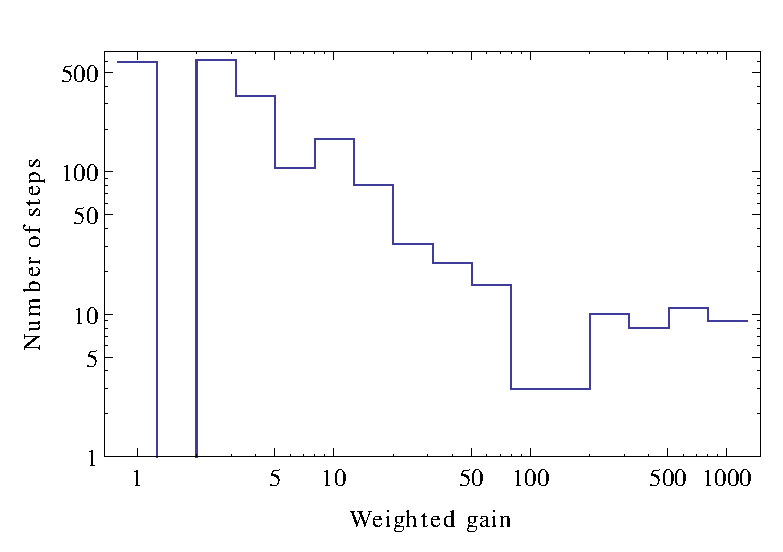
\includegraphics{student-kc-length-histogram.eps}
  \caption{Histogram of number of distinct student-KC pairs in student 
    dataset $\mathcal{A}$ having a given number of steps $N$.}
    \label{student-length-histogram}
\end{figure}

We examined log data from 12 students taking an intensive introductory
physics course at St.\ Anselm College during summer 2011.  The course
covered the same content as a normal two-semester introductory course.
Log data was recorded as students solved homework problems while using
the Andes intelligent tutor homework system.  231 hours of log data
were recorded.
%, covering 85,744 transactions, and 26,204 student steps.  
Each step was assigned to one or more different KC's.  The dataset
contains a total of 2017 distinct student-KC pairs covering a total of
245 distinct KC's.  We will refer to this dataset as student dataset
$\mathcal{A}$.  See Figure~\ref{student-length-histogram} for a
histogram of the number student-KC pairs having a given number of
steps.

Most KC's are associated with physics
or relevant math skills while others are associated with 
Andes conventions or user-interface actions (such as, notation
for defining a variable).  The student-KC pairs with the largest 
number of steps are associated with user-interface related skills,
since these skills are exercised throughout the entire course. 

The presence of many student-KC pairs with just one or two
steps may indicate that the default cognitive model associated 
with this tutor system may be sub-optimal; to date, there has not 
been any attempt, to date, to improve on the cognitive model of 
Andes with, say, Learning Factors Analysis~\cite{cen_learning_2006}.

\subsection{Analysis}

\begin{figure}
  \centering 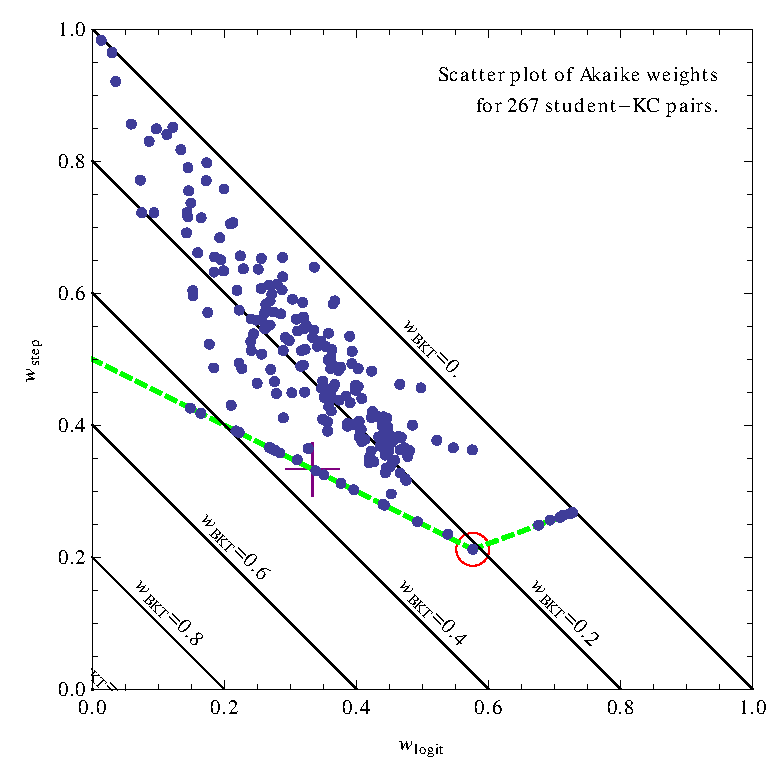
\includegraphics{scatter-weights.eps}
  \caption{Scatter plot of  Akaike weights for the three models, 
   $P_\mathrm{step}$, $P_\mathrm{logistic}$, and $P_\mathrm{BKT}$, 
   when fit to student-KC pairs from an introductory physics course.
   The point where all models are equal,
   $w_\mathrm{step}=w_\mathrm{logistic}=w_\mathrm{BKT}=1/3$, is
   marked with the lower cross.  
   The average of the  weights is marked with
   the upper cross.
  The dashed line on the left represents points
   where $w_\mathrm{step}=w_\mathrm{BKT}$.  Finally, the line on 
   the right marks data with bit strings of the form
   $00\cdots 011\cdots 1$.} 
   \label{scatter1}
\end{figure}

Since the goodness of fit criterion, AIC, is valid in the limit of
many steps, we include in this analysis only student-KC pairs that
contain 10 or more steps, reducing the number of student-KC pairs to
267, covering 38 distinct KC's.  We determine the correctness of each
step (Section~\ref{steps}), constructing a bit string, {\em exempli
gratia} 001001101, for each student-KC pair.  This bit string is then
fit to each of the three models, $P_\mathrm{step}$,
$P_\mathrm{logistic}$, and $P_\mathrm{BKT}$ by maximizing the
associated log likelihood.
%This determines the free parameters in each model. 
We then calculate the AIC score~\cite{burnham_model_2002} for each fit.  
Finally, we calculated the Akaike weights, $w_\mathrm{logistic}$, $w_\mathrm{step}$, and $w_\mathrm{BKT}$ for each student-KC pair.
The weights are normalized so that
%
\begin{equation}
   1=w_\mathrm{logistic}+ w_\mathrm{step} + w_\mathrm{BKT} \; .
\end{equation}
%
The Akaike weight represents the relative probability that
a particular model in a given set of models is closest
to the model that has actually generated the data. 

A scatter plot of the weights is shown in Fig.~\ref{scatter1}.
If all three models described the data equally well, then
we would expect points to be scattered evenly about 
center point $w_\mathrm{logistic}= w_\mathrm{step}= w_\mathrm{BKT}=1/3$.
Instead, we see the step model (average weight 0.44) weakly 
favored over the logistic model (average weight 0.37) and 
strongly favored over BKT (average weight 0.18).  Indeed, we 
find no data points where $w_\mathrm{step}< w_\mathrm{BKT}$,
although there is a noticable accumulation of points along the line 
$w_\mathrm{step}= w_\mathrm{BKT}$.

Note that data in the form of incorrect steps then correct steps, 
{\it exempli gratia}, $00\cdots 011\cdots 1$
is fit perfectly by both the $P_\mathrm{step}$ and 
$P_\mathrm{logistic}$ models.  
In this case, since $P_\mathrm{logistic}$ has one fewer parameter
than $P_\mathrm{step}$, it is favored by AIC by a constant factor and
$w_\mathrm{step}=\mathrm{e}^{-1} w_\mathrm{logistic}$.  This case is
plotted as the increasing dashed line in Fig.~\ref{scatter1}.

Since the student-KC pairs contain an average of about $N=16$ 
steps, it is surprising that we find that AIC so strongly
discriminates between the models.  Perhaps this is due to
some finite $N$ correction?  Recall that AIC is only 
strictly valid in the $N\to\infty$ limit.

\subsection{Random data}


\begin{figure}
  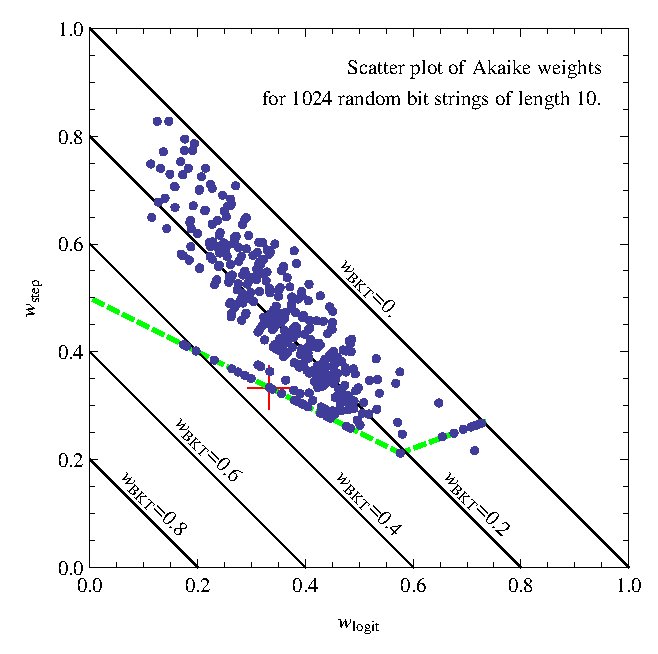
\includegraphics{scatter10.eps} \hfill
  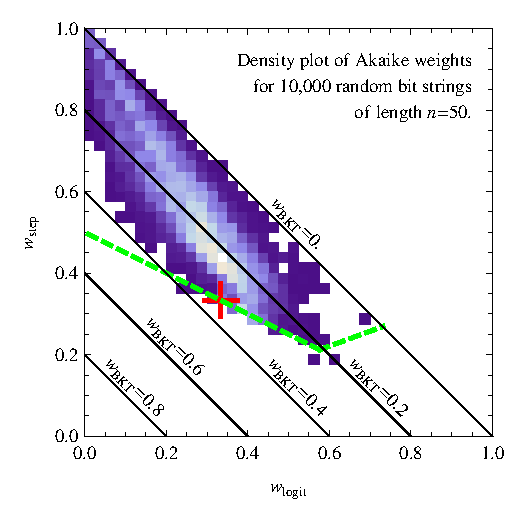
\includegraphics{density50.eps}
  \caption{Akaike weights for the three models, 
   $P_\mathrm{step}$, $P_\mathrm{logistic}$, and $P_\mathrm{BKT}$, 
   when fit to randomly generated data.  The point where
   $w_\mathrm{step}=w_\mathrm{logistic}=w_\mathrm{BKT}=1/3$ is
   marked with a cross.  For these datasets, each 
   model should perform equally well, since, with an appropriate
   choice of parameters, they all can be made equal to 
   the model that was used to generate the data.}\label{scatter2}
\end{figure}

To further investigate this situation, we constructed an
artificial dataset containing random bit strings (each
step has 50\% probability of being ``correct'') of length 
$N\in\left\{10,20,30,40,50\right\}$.
This dataset corresponds to a model of the form
%
\begin{equation}
        P_\mathrm{random}(j)=1/2 \; .
\end{equation}
%
We then repeated our analysis of the three models using this dataset
and AIC as our selection criterion.  Note that all three models,
with a suitable choice of parameters, can be made equal to 
$P_\mathrm{random}$.

As mentioned earlier, for data that is generated by a simple 
model ($P_\mathrm{random}$ is about as
simple as one can get) and the ``true'' model is included among
the set of models, BIC is the more appropriate criterion
for model selection~\cite[Sections~6.3 \& 6.4]{burnham_model_2002}.
However, the only difference between AIC and BIC for our results is that BIC favors
$P_\mathrm{logistic}$ more strongly over $P_\mathrm{step}$ and
$P_\mathrm{BKT}$.  Thus, using BIC would shift the weights so that
$w_\mathrm{logistic}$ would increase somewhat over the other two
models.  However, in order to maintain consistency with
our experimental results, Fig.~\ref{scatter1}, we will continue
to use AIC.  This use of AIC versus BIC will not affect our conclusions.

For data generated by $P_\mathrm{random}$,
one expects that all three models should perform equally
well since all three can equal (with suitable choice of parameters)
the known correct model $P_\mathrm{random}$.  Thus, we would expect
a scatter plot of the Akaike weights to center around
$w_\mathrm{logistic}=w_\mathrm{step}=w_\mathrm{BKT}=1/3$.  Instead, we
find that $P_\mathrm{step}$ is highly favored over the other two; see
Fig.~\ref{scatter2}. This bias seems to persist as we increase $N$.

\begin{figure}
   \centering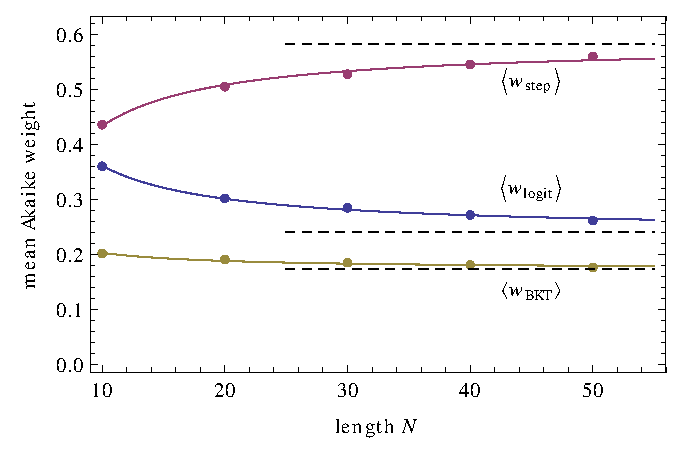
\includegraphics{mean-weights.eps}
  \caption{Mean Akaike weights for the three models, 
   $P_\mathrm{step}$, $P_\mathrm{logistic}$, and $P_\mathrm{BKT}$, 
   when fit to randomly generated data of length $N$.
   (Each mean is calculated by averaging over 10,000 random bit strings.)
   Also shown is a fit to a function of the form $a+b/N$ and
   a dashed line marking the asymptotic value $a$.
   Note that the differences between the weights persist
   in the $N\to\infty$ limit.}\label{meanweight}
\end{figure}

If we plot the average weight as a function of $N$, we find
that the differences between the weights persist
in the $N\to\infty$ limit;  see Fig.~\ref{meanweight}.
If we fit the average weights to a constant plus $1/N$;
the fits are:
%
\begin{eqnarray}
 \langle w_\mathrm{step}\rangle &=& 0.58 - \frac{1.50}{N} \\
 \langle w_\mathrm{logistic}\rangle &=& 0.24 + \frac{1.2}{N} \\
 \langle w_\mathrm{BKT}\rangle &=& 0.17+\frac{0.30}{N} \; .
\end{eqnarray}
%
This shows that AIC, in the asymptotic limit $N\to\infty$, 
still favors  $P_\mathrm{step}$ over the other two models
when used to evaluate randomly generated data.

If we repeat this analysis with BIC, we would also
find that the weights converge to a constant value with 
$1/N$ leading errors.  The only difference is that the logistic
model has a larger weight than the other two.  This is to be
expected since all three models contain the true model.

\subsection{Summary}

In conclusion, we obtain some suprising results when we compare
the three models,  $P_\mathrm{step}$, $P_\mathrm{logistic}$, and
$P_\mathrm{BKT}$.  The most remarkable result is that, for any bit
string,  $P_\mathrm{BKT}$ {\em never} fits the data better than $P_\mathrm{BKT}$.  Since 
both models have three parameters, this result holds for both
AIC and BIC.  We don't have an analytic proof explaining this result, 
but the numerical evidence (see Fig.~\ref{meanweight}) is quite strong.
It would be quite useful to better understand this result.

Second, we see that the scatter plot of Akaike weights for student
data is remarkably similar to the scatter plots for the random model.
This suggests that the student data has a high degree of randomness,
and that study of the random model may be quite useful for better
understanding the student data.

Third, tanking into account the fact that AIC seems to prefer the step model over the other
two for the random data (when we expect them to all work equally
well), we can still conclude that the step model works at least as
well as the other two for the student data.

Demonstrating that the step model fits student data as well as,
or better than, the other two would be an
{\em ex post facto} justification for using that model.  
However, our use of the step model is primarily motivated
by criteria~\ref{crit:step} and \ref{crit:perform} of 
Section~\ref{model-criteria}.
In Section~\ref{multi-model}, we show how AIC-based methods
can yield the probability that learning has occurred during given step.

\section{Multi-model approach}
\label{multi-model}

We need to determine the step where a specific student has learned a
particular skill.  Our strategy is to take the step model, 
$P_\mathrm{step}(j)$, and treat $L$ as a constant, yielding a set of $N$ 
sub-models $P_{\mathrm{step},L}(j)$, one for each value of $L$.
We then fit each of the $N$ sub-models to the student data and
calculate an AIC value.  Finally, we find the Akaike weighs for each of the
sub-models.  The Akaike weights give the relative probability that learning
occurred at each step.

\begin{figure}
  \centering 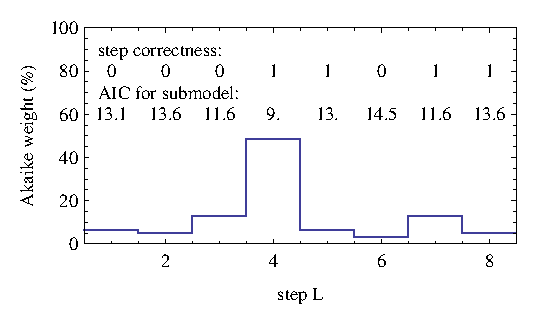
\includegraphics{step-weights.eps}
   \caption{Akaike weights for the submodels $P_\mathrm{step,L}(j)$.  
     This gives the relative probability that
      the student learned the KC just before step $L$.}
    \label{step-weights}
\end{figure}

Let us illustrate this technique with a simple example.  Suppose the
bit string for a particular student-KC pair is 00011011 (8
opportunities); see Fig.~\ref{step-weights}.  We fit this datum to 8
sub-models of the step model, corresponding to $L\in\{1,2,\ldots,8\}$,
by maximizing the log likelihood $\log\mathcal{L}$.  The associated
AIC values are given by $\mathrm{AIC}_L=2 K-\log \mathcal{L}$ where
$K$ is the number of fit parameters.  Note that there are two
parameters ($s$ and $g$) when $L>1$ and there is only one parameter
($s$) when $L=1$.
%
%\begin{table}
%\caption{
%\begin{tabular}{crrrrrrrr}
% opportunity & 1 & 2 & 3 &4 & 5 & 6 & 7 & 8 \\
 % AIC &   13.1 & 13.6 & 11.6 & 9.0 & 13.0 & 14.5 & 11.6 & 13.6 \\
%\end{tabular}
%\end{equation}
%
Not suprisingly, the best fit (lowest AIC) corresponds to the first
``1'' in the bit string at step~4.  From the AICs, we calculate 
the Akaike weights
%
\begin{equation}
     w_L=\frac{e^{-\mathrm{AIC}_L/2} }{\sum_{L^\prime}
       e^{-\mathrm{AIC}_{L^\prime}/2}} \; .
\end{equation}
%
The Akaike weight $w_L$ gives the relative probability that sub-model 
$P_{\mathrm{step},L}(j)$ is, of all the sub-models, the closest to the 
the model that actually generated the data.


Note that the case $L=1$ corresponds to the student having 
``learned the skill'' some time before the first step.  That is to say, 
the student does not acquire the skill while using the tutor system.
Thus, $w_1$ should be interpreted as the relative probability
that no learning has occurred while using the tutor system.

\section{Weighted gain}

Our ultimate goal is to distinguish steps that result in 
learning from steps that do not.  Hopefully, one can use this
information to infer something about the effectiveness of the help
given on a particular step, or the effectiveness of
the student activity on that step.

\begin{figure}
  \centering 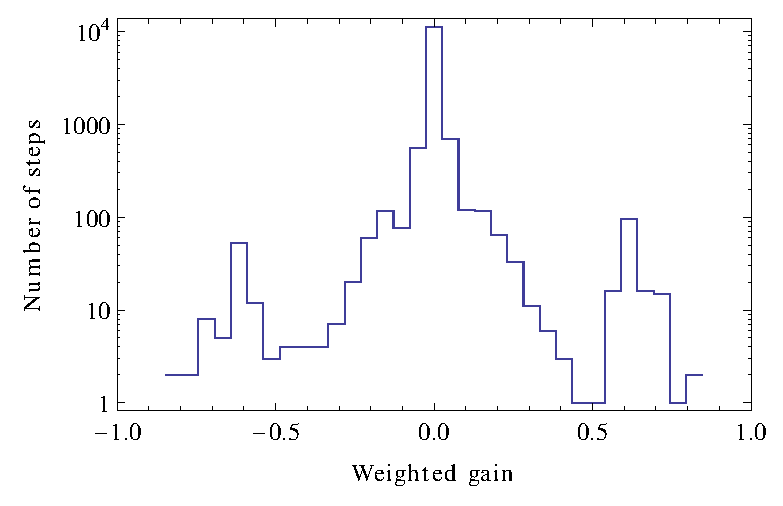
\includegraphics{weighted-gain-histogram.eps}
   \caption{Histogram of weighted gains $w_L \Delta_L$ for
     all steps in all student-KC pairs in student dataset $\mathcal{A}$.}
    \label{weighted-gain-histogram}
\end{figure}

It is not sufficient to know {\it when} learning has occurred but one
must also determine {\it how much} learning has occurred.  Consider
the bit sequence 11011000.  When fit to the step model, the best fit
will occur at $L=6$ but this would correspond to a decrease in student
performance for that skill.  In other cases, the change in student
performance may be almost zero.  In order to take this into account,
we propose using the Akaike weight $w_L$ times the associated learning
gain $\Delta_L$ to characterize a step.  We define the learning gain
$\Delta_L=1-\hat{g}-\hat{s}$ where $\hat{g}$ and $\hat{s}$ are the
Maximum Likelihood estimators for $g$ and $s$ given by submodel
$P_{\mathrm{step},L}(j)$.  For the ``no learning'' case $L=1$, we set
$\Delta_1=0$.  We will call $w_L \Delta_L$ the ``weighted gain''
associated with $P_{\mathrm{step},L}(j)$.  A histogram of $w_L
\Delta_L$ for student dataset $\mathcal{A}$ is shown in
Fig.~\ref{weighted-gain-histogram}.  Note that the vast majority of
steps (29730) have almost zero weighted gain.  We also see that there
is a significant number of steps with negative gain (988), but there
are somewhat more steps with positive gain (1312) .

The fact that there are so many steps with negative gain is
symptomatic of bit strings that are very noisy (a lot of
randomness).  Indeed, if we compare the histogram for student
dataset $\mathcal{A}$ with the histogram for a randomly 
generated dataset $\mathcal{R}$ (we take $\mathcal{A}$ and
randomly permute the steps) we find a similar distribution;
see Fig.~\ref{weighted-gain-histogram2}.

What would the distribution look like if the data weren't 
so noisy?  To see this, we generated an artificial ``ideal'' dataset
$\mathcal{I}$ where there were no slips or guesses, but having
the same length distribution as $\mathcal{A}$ 
(Fig.~\ref{student-length-histogram}).  Thus, the bit strings
in $\mathcal{I}$ have the form $00\cdots011\cdots1$.
In this case, for each student-KC pair, we expect a single 
large weighted gain (corresponding to the first 1 in the bit string) 
and the remaining weighted gains to be nearly zero.  The resulting 
distribution of gains is shown
in  Fig.~\ref{weighted-gain-histogram2}.

\begin{figure}
  \centering 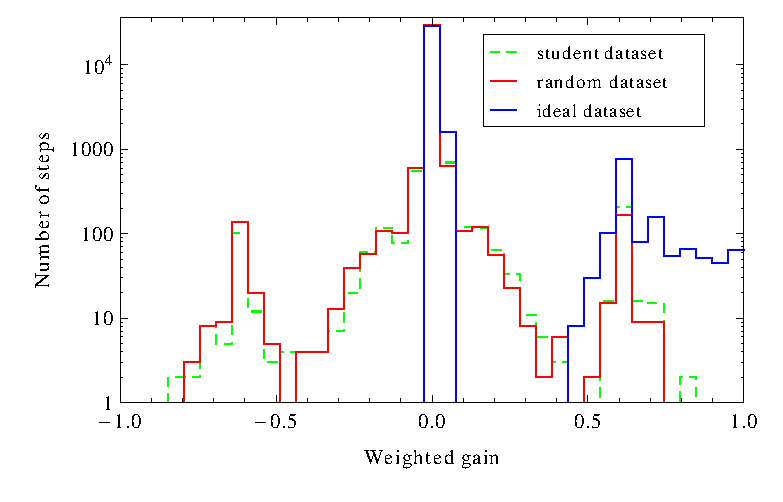
\includegraphics{weighted-gain-histogram2.eps}
   \caption{Histogram of weighted gains $w_L \Delta_L$ for
     the student dataset $\mathcal{A}$, 
     a randomly generated dataset $\mathcal{R}$,
     and an artificial ideal dataset $\mathcal{I}$.}
    \label{weighted-gain-histogram2}
\end{figure}


We propose to use the following average of the weighed gains as
a ``quality index'' for determining how suitable a 
dataset is for determining the point of learning for an individual
student-KC pair:
%
\begin{equation}
           Q= \frac{1}{N} \sum_\alpha \sum_L w_L \Delta_L
\end{equation}
%
where $\alpha$ is an index running over all student-KC pairs in a 
dataset and $N$ is the number of student-KC pairs.
We use the sample standard deviation of the weighted gains $w_L \Delta_L$
to calculate the standard error associated with $Q$. 

For the random dataset $\mathcal{R}$, we expect the distribution of
weighted gains to be symmetric about zero and thus $Q$ to approach
zero.  Numerically, we find $Q=-0.002\pm0.002$, consistent with zero.
For the ``ideal'' dataset $\mathcal{I}$, we expect, for the first 1 in
the bit string, $w_L$ to be nearly one with the associated $\Delta_L$
also nearly one so that $Q\to 1$ in the limit of many opportunities.
Numerically, we obtain $Q=0.5240\pm0.0003$.  The fact that it is much
smaller than one is due to the large number of student-KC pairs having
just a few steps.  For the student dataset $\mathcal{A}$, we obtain
$Q=0.0467\pm0.0065$, which is small, but significant
($p<0.001$). Thus, we conclude that the student dataset is of
sufficient quality to use in determining where learning has occurred.


\section{Conclusion}

It is clear that determining the moment of learning for an
individual student is a murky business.  As can be seen in
Fig.~\ref{weighted-gain-histogram2}, there is not much difference
between a student dataset and a randomly generated dataset.  We have
introduced the quality index $Q$ which can be used to quantify the
size of the signal as well as the size of the background.  We see that
$Q=0.0467\pm0.0065$ for the student dataset $\mathcal{A}$ is roughly
10\% the size of $Q$ for the ideal dataset $\mathcal{I}$; we interpret
this to mean that the ``signal'' is rougly 10\% as big as the
``noise.''  However, the fact that $Q$ for the student dataset is
seven standard deviations from zero means that we have detected
learning for 2000 student-KC pairs with room to spare.  Using the fact
that the error goes as $1/\sqrt{n}$, where $n$ is the number 
of student-KC pairs, we estimate
that we could still detect learning with only 260 student-KC pairs at the
$p=0.01$ level.  This gives us an initial estimate for the amount of
log data needed to measure the moment of learning, at least for
students using the Andes tutor system.

As seen in Fig.~\ref{student-length-histogram}, we see that many of
the student-KC pairs are quite short.  We speculate that this
is due to to the way that physics is typically taught, with relatively
little reinforcement of specific KCs, emphasizing, instead, more
general problem solving meta-skills.  If we were to repeat this
analysis for high school or grade school math, where there is more
repitition, we speculate that there would be significantly fewer KCs
with less than 10 opportunities and that detecting when learning has
occurred would be significantly easier.


% Bibliography
\bibliographystyle{acmlarge}
\bibliography{education-modeling}



\end{document}